% Options for packages loaded elsewhere
\PassOptionsToPackage{unicode}{hyperref}
\PassOptionsToPackage{hyphens}{url}
%
\documentclass[
  a4paper,
]{scrbook}

\usepackage{amsmath,amssymb}
\usepackage[]{accanthis}
\usepackage{iftex}
\ifPDFTeX
  \usepackage[T1]{fontenc}
  \usepackage[utf8]{inputenc}
  \usepackage{textcomp} % provide euro and other symbols
\else % if luatex or xetex
  \usepackage{unicode-math}
  \defaultfontfeatures{Scale=MatchLowercase}
  \defaultfontfeatures[\rmfamily]{Ligatures=TeX,Scale=1}
\fi
% Use upquote if available, for straight quotes in verbatim environments
\IfFileExists{upquote.sty}{\usepackage{upquote}}{}
\IfFileExists{microtype.sty}{% use microtype if available
  \usepackage[]{microtype}
  \UseMicrotypeSet[protrusion]{basicmath} % disable protrusion for tt fonts
}{}
\makeatletter
\@ifundefined{KOMAClassName}{% if non-KOMA class
  \IfFileExists{parskip.sty}{%
    \usepackage{parskip}
  }{% else
    \setlength{\parindent}{0pt}
    \setlength{\parskip}{6pt plus 2pt minus 1pt}}
}{% if KOMA class
  \KOMAoptions{parskip=half}}
\makeatother
\usepackage{xcolor}
\setlength{\emergencystretch}{3em} % prevent overfull lines
\setcounter{secnumdepth}{5}
% Make \paragraph and \subparagraph free-standing
\ifx\paragraph\undefined\else
  \let\oldparagraph\paragraph
  \renewcommand{\paragraph}[1]{\oldparagraph{#1}\mbox{}}
\fi
\ifx\subparagraph\undefined\else
  \let\oldsubparagraph\subparagraph
  \renewcommand{\subparagraph}[1]{\oldsubparagraph{#1}\mbox{}}
\fi
\pagestyle{headings}

\usepackage{color}
\usepackage{fancyvrb}
\newcommand{\VerbBar}{|}
\newcommand{\VERB}{\Verb[commandchars=\\\{\}]}
\DefineVerbatimEnvironment{Highlighting}{Verbatim}{commandchars=\\\{\}}
% Add ',fontsize=\small' for more characters per line
\newenvironment{Shaded}{}{}
\newcommand{\AlertTok}[1]{\textcolor[rgb]{1.00,0.33,0.33}{\textbf{#1}}}
\newcommand{\AnnotationTok}[1]{\textcolor[rgb]{0.42,0.45,0.49}{#1}}
\newcommand{\AttributeTok}[1]{\textcolor[rgb]{0.84,0.23,0.29}{#1}}
\newcommand{\BaseNTok}[1]{\textcolor[rgb]{0.00,0.36,0.77}{#1}}
\newcommand{\BuiltInTok}[1]{\textcolor[rgb]{0.84,0.23,0.29}{#1}}
\newcommand{\CharTok}[1]{\textcolor[rgb]{0.01,0.18,0.38}{#1}}
\newcommand{\CommentTok}[1]{\textcolor[rgb]{0.42,0.45,0.49}{#1}}
\newcommand{\CommentVarTok}[1]{\textcolor[rgb]{0.42,0.45,0.49}{#1}}
\newcommand{\ConstantTok}[1]{\textcolor[rgb]{0.00,0.36,0.77}{#1}}
\newcommand{\ControlFlowTok}[1]{\textcolor[rgb]{0.84,0.23,0.29}{#1}}
\newcommand{\DataTypeTok}[1]{\textcolor[rgb]{0.84,0.23,0.29}{#1}}
\newcommand{\DecValTok}[1]{\textcolor[rgb]{0.00,0.36,0.77}{#1}}
\newcommand{\DocumentationTok}[1]{\textcolor[rgb]{0.42,0.45,0.49}{#1}}
\newcommand{\ErrorTok}[1]{\textcolor[rgb]{1.00,0.33,0.33}{\underline{#1}}}
\newcommand{\ExtensionTok}[1]{\textcolor[rgb]{0.84,0.23,0.29}{\textbf{#1}}}
\newcommand{\FloatTok}[1]{\textcolor[rgb]{0.00,0.36,0.77}{#1}}
\newcommand{\FunctionTok}[1]{\textcolor[rgb]{0.44,0.26,0.76}{#1}}
\newcommand{\ImportTok}[1]{\textcolor[rgb]{0.01,0.18,0.38}{#1}}
\newcommand{\InformationTok}[1]{\textcolor[rgb]{0.42,0.45,0.49}{#1}}
\newcommand{\KeywordTok}[1]{\textcolor[rgb]{0.84,0.23,0.29}{#1}}
\newcommand{\NormalTok}[1]{\textcolor[rgb]{0.14,0.16,0.18}{#1}}
\newcommand{\OperatorTok}[1]{\textcolor[rgb]{0.14,0.16,0.18}{#1}}
\newcommand{\OtherTok}[1]{\textcolor[rgb]{0.44,0.26,0.76}{#1}}
\newcommand{\PreprocessorTok}[1]{\textcolor[rgb]{0.84,0.23,0.29}{#1}}
\newcommand{\RegionMarkerTok}[1]{\textcolor[rgb]{0.42,0.45,0.49}{#1}}
\newcommand{\SpecialCharTok}[1]{\textcolor[rgb]{0.00,0.36,0.77}{#1}}
\newcommand{\SpecialStringTok}[1]{\textcolor[rgb]{0.01,0.18,0.38}{#1}}
\newcommand{\StringTok}[1]{\textcolor[rgb]{0.01,0.18,0.38}{#1}}
\newcommand{\VariableTok}[1]{\textcolor[rgb]{0.89,0.38,0.04}{#1}}
\newcommand{\VerbatimStringTok}[1]{\textcolor[rgb]{0.01,0.18,0.38}{#1}}
\newcommand{\WarningTok}[1]{\textcolor[rgb]{1.00,0.33,0.33}{#1}}

\providecommand{\tightlist}{%
  \setlength{\itemsep}{0pt}\setlength{\parskip}{0pt}}\usepackage{longtable,booktabs,array}
\usepackage{calc} % for calculating minipage widths
% Correct order of tables after \paragraph or \subparagraph
\usepackage{etoolbox}
\makeatletter
\patchcmd\longtable{\par}{\if@noskipsec\mbox{}\fi\par}{}{}
\makeatother
% Allow footnotes in longtable head/foot
\IfFileExists{footnotehyper.sty}{\usepackage{footnotehyper}}{\usepackage{footnote}}
\makesavenoteenv{longtable}
\usepackage{graphicx}
\makeatletter
\def\maxwidth{\ifdim\Gin@nat@width>\linewidth\linewidth\else\Gin@nat@width\fi}
\def\maxheight{\ifdim\Gin@nat@height>\textheight\textheight\else\Gin@nat@height\fi}
\makeatother
% Scale images if necessary, so that they will not overflow the page
% margins by default, and it is still possible to overwrite the defaults
% using explicit options in \includegraphics[width, height, ...]{}
\setkeys{Gin}{width=\maxwidth,height=\maxheight,keepaspectratio}
% Set default figure placement to htbp
\makeatletter
\def\fps@figure{htbp}
\makeatother
\newlength{\cslhangindent}
\setlength{\cslhangindent}{1.5em}
\newlength{\csllabelwidth}
\setlength{\csllabelwidth}{3em}
\newlength{\cslentryspacingunit} % times entry-spacing
\setlength{\cslentryspacingunit}{\parskip}
\newenvironment{CSLReferences}[2] % #1 hanging-ident, #2 entry spacing
 {% don't indent paragraphs
  \setlength{\parindent}{0pt}
  % turn on hanging indent if param 1 is 1
  \ifodd #1
  \let\oldpar\par
  \def\par{\hangindent=\cslhangindent\oldpar}
  \fi
  % set entry spacing
  \setlength{\parskip}{#2\cslentryspacingunit}
 }%
 {}
\usepackage{calc}
\newcommand{\CSLBlock}[1]{#1\hfill\break}
\newcommand{\CSLLeftMargin}[1]{\parbox[t]{\csllabelwidth}{#1}}
\newcommand{\CSLRightInline}[1]{\parbox[t]{\linewidth - \csllabelwidth}{#1}\break}
\newcommand{\CSLIndent}[1]{\hspace{\cslhangindent}#1}


\usepackage{titling}
\setlength{\droptitle}{-2cm}
\preauthor{
  \begin{center}
  
\includegraphics[width=5in,height=4in]{cover.png}\\ % cover figure
  \Large
}
\postauthor{
  \end{center}
}
\predate{
  \begin{center}
  Master of Science in Biology\\               % Degree
  Biodiversity, Evolution and Ecology\\        % Degree stream
  Department of Biological Sciences\\          % Department
  University of Bergen\\                       % University 
  \vspace{5mm}
}
\postdate{
  \\
  
\includegraphics[width=1.5in,height=1.5in]{figures/anr-dfg.jpg}\\
  \end{center}
  \newpage
  \mbox{}
  \vfill
  Cover page\\
  \emph{Beckwithia glacialis} on Snøhetta.
 }
<script type="ojs-define">
{"contents":[{"name":"data","value":{"year":["1958","1959","1960"],"max":[317.51,318.29,320.04]}}]}
</script>
\makeatletter
\makeatother
\makeatletter
\@ifpackageloaded{caption}{}{\usepackage{caption}}
\AtBeginDocument{%
\ifdefined\contentsname
  \renewcommand*\contentsname{Table of contents}
\else
  \newcommand\contentsname{Table of contents}
\fi
\ifdefined\listfigurename
  \renewcommand*\listfigurename{List of Figures}
\else
  \newcommand\listfigurename{List of Figures}
\fi
\ifdefined\listtablename
  \renewcommand*\listtablename{List of Tables}
\else
  \newcommand\listtablename{List of Tables}
\fi
\ifdefined\figurename
  \renewcommand*\figurename{Figure}
\else
  \newcommand\figurename{Figure}
\fi
\ifdefined\tablename
  \renewcommand*\tablename{Table}
\else
  \newcommand\tablename{Table}
\fi
}
\@ifpackageloaded{float}{}{\usepackage{float}}
\floatstyle{ruled}
\@ifundefined{c@chapter}{\newfloat{codelisting}{h}{lop}}{\newfloat{codelisting}{h}{lop}[chapter]}
\floatname{codelisting}{Listing}
\newcommand*\listoflistings{\listof{codelisting}{List of Listings}}
\makeatother
\makeatletter
\@ifpackageloaded{caption}{}{\usepackage{caption}}
\@ifpackageloaded{subcaption}{}{\usepackage{subcaption}}
\makeatother
\makeatletter
\@ifpackageloaded{tcolorbox}{}{\usepackage[many]{tcolorbox}}
\makeatother
\makeatletter
\@ifundefined{shadecolor}{\definecolor{shadecolor}{rgb}{.97, .97, .97}}
\makeatother
\makeatletter
\makeatother
\ifLuaTeX
  \usepackage{selnolig}  % disable illegal ligatures
\fi
\IfFileExists{bookmark.sty}{\usepackage{bookmark}}{\usepackage{hyperref}}
\IfFileExists{xurl.sty}{\usepackage{xurl}}{} % add URL line breaks if available
\urlstyle{same} % disable monospaced font for URLs
\hypersetup{
  pdftitle={Gestion d'une base de donnée qualitatives et géometrique},
  pdfauthor={Elina Marveaux},
  hidelinks,
  pdfcreator={LaTeX via pandoc}}

\title{Gestion d'une base de donnée qualitatives et géometrique}
\author{Elina Marveaux}
\date{12/05/2022}

\begin{document}
\frontmatter
\maketitle
\ifdefined\Shaded\renewenvironment{Shaded}{\begin{tcolorbox}[breakable, sharp corners, frame hidden, borderline west={3pt}{0pt}{shadecolor}, enhanced, interior hidden, boxrule=0pt]}{\end{tcolorbox}}\fi

\renewcommand*\contentsname{Table des matières}
{
\setcounter{tocdepth}{2}
\tableofcontents
}
\listoffigures
\listoftables
\mainmatter
\hypertarget{preface}{%
\chapter*{Preface}\label{preface}}
\addcontentsline{toc}{chapter}{Preface}

This is a Quarto book.

To learn more about Quarto books visit
\url{https://quarto.org/docs/books}.

\begin{verbatim}
[1] 2
\end{verbatim}

\begin{figure}

{\centering 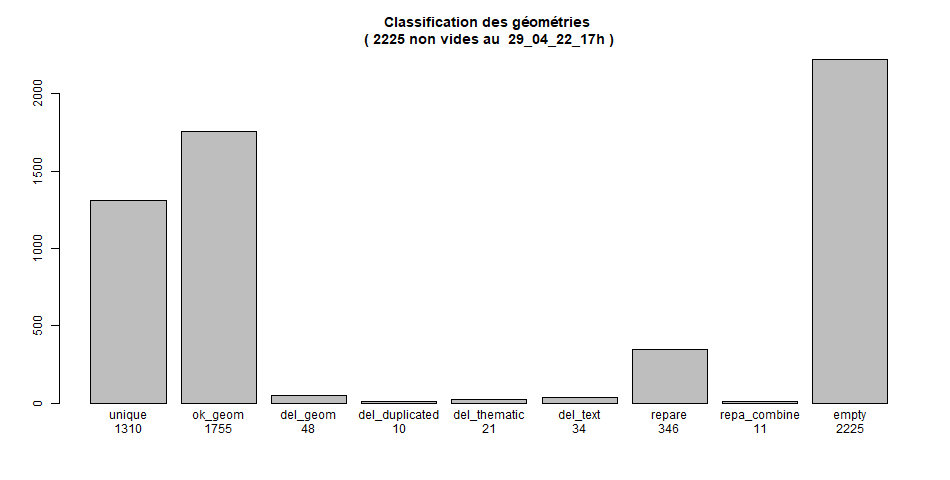
\includegraphics{./figures/bar_classify_Del_29_04_22_17h.png}

}

\caption{Chart Bar des NAS}

\end{figure}

\hypertarget{summary}{%
\chapter{Summary}\label{summary}}

In summary, this book has no content whatsoever.

\begin{verbatim}
[1] 2
\end{verbatim}

\hypertarget{introduction}{%
\chapter{Introduction}\label{introduction}}

R table

\begin{Shaded}
\begin{Highlighting}[numbers=left,,]
\NormalTok{data }\OtherTok{\textless{}{-}} \FunctionTok{data.frame}\NormalTok{(}\AttributeTok{year =}  \FunctionTok{c}\NormalTok{(}\StringTok{"1958"}\NormalTok{, }\StringTok{"1959"}\NormalTok{, }\StringTok{"1960"}\NormalTok{), }
                   \AttributeTok{max =} \FunctionTok{c}\NormalTok{(}\FloatTok{317.51}\NormalTok{, }\FloatTok{318.29}\NormalTok{, }\FloatTok{320.04}\NormalTok{))}

\FunctionTok{ojs\_define}\NormalTok{(data)}

\NormalTok{data}
\end{Highlighting}
\end{Shaded}

\begin{verbatim}
  year    max
1 1958 317.51
2 1959 318.29
3 1960 320.04
\end{verbatim}

\texttt{OJS} line\_chart from tutorial with \texttt{ojs\_define()} and
\texttt{R} table

\begin{Shaded}
\begin{Highlighting}[numbers=left,,]
\NormalTok{tableR = data}
\NormalTok{tableOjs = transpose(tableR)}

\NormalTok{tableOjs}

\NormalTok{yearlyChart = Plot.plot(\{}
\NormalTok{  marks: [}
\NormalTok{    Plot.line(tableOjs, }
\NormalTok{      \{x: "year", y: "max"\}, }
\NormalTok{      \{ stroke: "red" \}}
\NormalTok{    )}
\NormalTok{  ]\}}
\NormalTok{)}
\end{Highlighting}
\end{Shaded}

Second bar chart

\begin{Shaded}
\begin{Highlighting}[numbers=left,,]

\NormalTok{Plot.rectY(tableOjs, Plot.binX(\{y: "max"\}, \{x: "year"\})).plot()}
\end{Highlighting}
\end{Shaded}

Third bar chart with \texttt{python} table

\begin{Shaded}
\begin{Highlighting}[numbers=left,,]
\NormalTok{Plot.plot(\{}
\NormalTok{  marks: [}
\NormalTok{    Plot.barY(tableOjs, \{x: "year", y: "max"\})}
\NormalTok{  ]}
\NormalTok{\})}
\end{Highlighting}
\end{Shaded}

\hypertarget{penguins}{%
\chapter{``Penguins''}\label{penguins}}

A simple example based on Allison Horst's
\href{https://allisonhorst.github.io/palmerpenguins/}{Palmer Penguins}
dataset. Here we look at how penguin body mass varies across both sex
and species (use the provided inputs to filter the dataset by bill
length and island):

\begin{Shaded}
\begin{Highlighting}[numbers=left,,]
\NormalTok{//| echo = false}
\NormalTok{data = FileAttachment("data/palmer{-}penguins.csv").csv(\{ typed: true \})}
\end{Highlighting}
\end{Shaded}

\begin{Shaded}
\begin{Highlighting}[numbers=left,,]
\NormalTok{//| echo = false}
\NormalTok{viewof bill\_length\_mm = Inputs.range(}
\NormalTok{  [32, 50], }
\NormalTok{  \{value: 35, step: 1, label: "Bill length (min):"\}}
\NormalTok{)}
\NormalTok{viewof islands = Inputs.checkbox(}
\NormalTok{  ["Torgersen", "Biscoe", "Dream"], }
\NormalTok{  \{ value: ["Torgersen", "Biscoe"], }
\NormalTok{    label: "Islands:"}
\NormalTok{  \}}
\NormalTok{)}
\end{Highlighting}
\end{Shaded}

\begin{Shaded}
\begin{Highlighting}[numbers=left,,]
\NormalTok{//| echo: false}
\NormalTok{filtered = data.filter(function(penguin) \{}
\NormalTok{  return bill\_length\_mm \textless{} penguin.bill\_length\_mm \&\&}
\NormalTok{         islands.includes(penguin.island);}
\NormalTok{\})}
\end{Highlighting}
\end{Shaded}

\hypertarget{plot}{%
\section{Plot}\label{plot}}

\begin{Shaded}
\begin{Highlighting}[numbers=left,,]
\NormalTok{//| echo: false}
\NormalTok{//| output: true}
\NormalTok{//| label: fig{-}penguin{-}body{-}mass}
\NormalTok{//| fig{-}cap: "Penguin body mass by sex and species"}
\NormalTok{Plot.rectY(filtered, }
\NormalTok{  Plot.binX(}
\NormalTok{    \{y: "count"\}, }
\NormalTok{    \{x: "body\_mass\_g", fill: "species", thresholds: 20\}}
\NormalTok{  ))}
\NormalTok{  .plot(\{}
\NormalTok{    facet: \{}
\NormalTok{      data: filtered,}
\NormalTok{      x: "sex",}
\NormalTok{      y: "species",}
\NormalTok{      marginRight: 80}
\NormalTok{    \},}
\NormalTok{    marks: [}
\NormalTok{      Plot.frame(),}
\NormalTok{    ]}
\NormalTok{  \}}
\NormalTok{)}
\end{Highlighting}
\end{Shaded}

\hypertarget{data}{%
\section{Data}\label{data}}

The \texttt{penguins} data from the
\href{https://allisonhorst.github.io/palmerpenguins}{\textbf{palmerpenguins}}
package contains size measurements for 344 penguins from three species
observed on three islands in the Palmer Archipelago, Antarctica./ The
plot below shows the relationship between flipper and bill lengths of
these penguins.

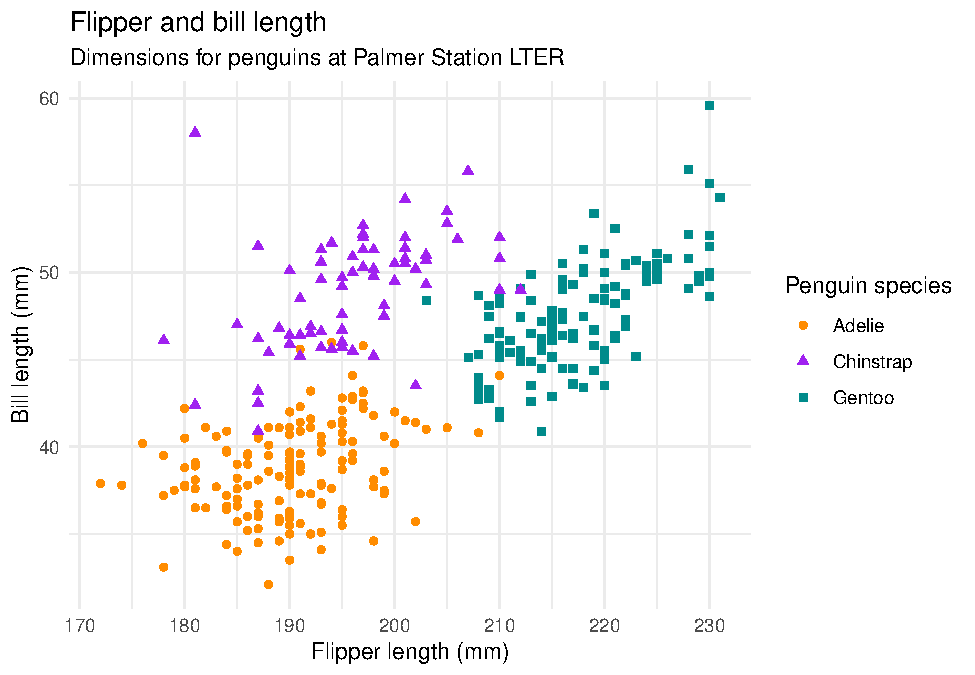
\includegraphics{./part1_files/figure-pdf/plot-penguins-1.pdf}

\hypertarget{references}{%
\chapter*{References}\label{references}}
\addcontentsline{toc}{chapter}{References}

\hypertarget{refs}{}
\begin{CSLReferences}{0}{0}
\end{CSLReferences}

\hypertarget{summary-1}{%
\chapter{Summary}\label{summary-1}}

In summary, this book has no content whatsoever.

\begin{verbatim}
[1] 2
\end{verbatim}

\appendix
\addcontentsline{toc}{part}{Appendices}

\hypertarget{sec-more-results}{%
\chapter{More results}\label{sec-more-results}}

Some results that wouldn't fit into the main thesi

Some results that wouldn't fit into the main thesis

\begin{figure}

{\centering 
\includegraphics{./cover.png}

}

\caption{cover}

\end{figure}


\backmatter

\end{document}
